\section{IDXL Communication}

The FEM framework's communication layer is called IDXL. This small library handles sending and receiving data to and from a sparse subset of 1D indices into a user array.  The sparse index subset is called an "Index List", hence the name of the library.


\subsection{Index Lists}
\label{sec:IDXL}
An Index List is the fundamental data structure of the IDXL library---for example, the list of shared nodes is an Index List.  IDXL includes routines for building, combining, and sending and receiving Index Lists.

An Index List, as you might expect, is a list of indices that need to be sent and received.  An Index List includes both the indices that need to be sent, as well as the indices to be received, from each chunk.

Consider two chunks $a$ and $b$ where $b$ needs some information $a$ has, such as if $b$ has ghosts of real elements on $a$.  $a$'s Index List thus has a send portion with the $a$-local indices for the elements $a$ sends; and $b$'s Index List contains a receive portion with the $b$-local indices for the elements $b$ receives.  Thus across processors, the corresponding send and receive portions of $a$ and $b$'s Index Lists match, as shown in Figure~\ref{fig:indexlists}.


\begin{figure}[h]
\begin{center}
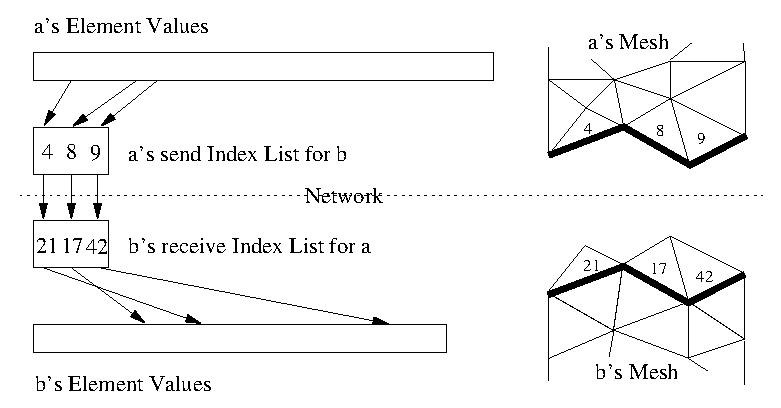
\includegraphics[width=5in]{fig/indexlists}
\end{center}
\caption{Illustrating how Index Lists match up $a$'s source elements with $b$'s ghost elements.}
\label{fig:indexlists}
\end{figure}



%%%%%%%%%%%%%%%%%%% Index Lists %%%%%%%%%%%%%%%%%%%%
\subsubsection{Index List Calls}

You refer to an Index List via an opaque handle---in C, the integer typedef \kw{IDXL\_t}; in Fortran, a bare INTEGER.  


\prototype{FEM\_Comm\_shared}
\function{IDXL\_t FEM\_Comm\_shared(int mesh,int entity);}
\function{INTEGER function FEM\_Comm\_shared(mesh,entity)}
  \args{INTEGER, INTENT(IN)  :: mesh,entity}

Return a read-only copy of the Index List of shared nodes.  The send and receive portions of this list are identical, because each shared node is both sent and received.  Shared nodes are most often used with the \kw{send/sum} communication pattern.

Must be called from driver.  \kw{mesh} must be a reading mesh. \kw{entity} must be \kw{FEM\_NODE}.  You may not call \kw{IDXL\_Destroy} on the returned list.


\prototype{FEM\_Comm\_ghost}
\function{IDXL\_t FEM\_Comm\_ghost(int mesh,int entity);}
\function{INTEGER function FEM\_Comm\_ghost(mesh,entity)}
  \args{INTEGER, INTENT(IN)  :: mesh,entity}

Return a read-only copy of the Index List of ghost entities.  The send portion of this list contains real, interior entities, which are sent away; the receive portion of the list contains the ghost entites, which are received. Ghosts are most often used with the \kw{send/recv} communication pattern.

Elements to be sent out are listed starting at zero (one in Fortran); but ghost elements to be received are also listed starting at zero (one in Fortran).  If real and ghost elements are kept in separate arrays, this is usable as-is; but if ghosts and real elements are kept together, you will need to shift the ghost indices using \kw{IDXL\_Combine} or \kw{IDXL\_Shift}. 

This routine must be called from driver.  \kw{mesh} must be a reading mesh. \kw{entity} must not include \kw{FEM\_GHOST}--ghosts are already included.  You may not call \kw{IDXL\_Destroy} on the returned list.


\prototype{IDXL\_Create}
\function{IDXL\_t IDXL\_Create(void);}
\function{INTEGER function IDXL\_Create()}

Create a new, empty Index List. This list can then be filled up using \kw{IDXL\_Copy} or \kw{IDXL\_Combine}.

Must be called from driver.  You must eventually call \kw{IDXL\_Destroy} on the returned list.


\prototype{IDXL\_Combine}
\function{void IDXL\_Combine(IDXL\_t dest,IDXL\_t src,int startSend,int startRecv);}
\function{SUBROUTINE IDXL\_Combine(dest,src,startSend,startRecv)}
  \args{INTEGER, INTENT(IN)  :: dest,src,startSend,startRecv}

Add the shifted contents of the src Index List to dest.  The send portion of src is shifted so the first index sent will be startSend; for a ghost index list this is the index of the first sent real entity. The receive portion of src is similarly shifted so the first index received will be startRecv; for a ghost index list this is the index of the first received ghost entity.  

This routine does not check for duplicates---if an index originally appears in dest and the also in the shifted src, it will be listed twice.


\subsubsection{Advanced Index List Calls}

\prototype{IDXL\_Destroy}
\function{void IDXL\_Destroy(IDXL\_t l);}
\function{SUBROUTINE IDXL\_Destroy(l)}
  \args{INTEGER, INTENT(IN)  :: l}

Destroy this Index List, and free the list storage allocated by the framework.  Only call this routine with lists you created using \kw{IDXL\_Create}; not lists obtained directly from the FEM framework.

\prototype{IDXL\_Print}
\function{void IDXL\_Print(IDXL\_t l);}
\function{SUBROUTINE IDXL\_Print(l)}
  \args{INTEGER, INTENT(IN)  :: l}

Print out the contents of this Index List.  This routine shows both the send and receive indices on the list, for each chunk we communicate with.


\prototype{IDXL\_Copy}
\function{void IDXL\_Copy(IDXL\_t dest,IDXL\_t src);}
\function{SUBROUTINE IDXL\_Print(dest,src)}
  \args{INTEGER, INTENT(IN)  :: dest,src}

Copy the contents of the source Index List into the destination Index List, which should be empty.

\prototype{IDXL\_Shift}
\function{void IDXL\_Shift(IDXL\_t l,int startSend,int startRecv);}
\function{SUBROUTINE IDXL\_Shift(l,startSend,startRecv)}
  \args{INTEGER, INTENT(IN)  :: l,startSend,startRecv}

Like \kw{IDXL\_Combine}, but only shifts the indices within a single list.


\prototype{IDXL\_Add\_entity}
\function{void IDXL\_Add\_entity(int newIdx,int nBetween,int *between);}
\function{SUBROUTINE IDXL\_Add\_node(newIdx,nBetween,between)}
    \args{INTEGER, INTENT(IN) :: newIdx,nBetween}
    \args{INTEGER, INTENT(IN) :: between(nBetween)}

This call adds a new entity, with local index \kw{newIdx}, to this Index List.  The new entity is sent or received by each chunk that sends or receives all the entites listed in the between array.  For example, when adding a new node along an edge, nBetween is 2 and between lists the endpoints of the edge; this way if the edge is shared with some chunk, the new node will be shared with that chunk.

This routine only affects the current chunk-- no other chunks are affected.  To ensure the communication lists match, \kw{IDXL\_Add\_entity} must be called on all the chunks that send or receive the entity, to create the local copies of the entity.

\kw{IDXL\_Add\_entity} adds the new entity to the end of the communication list, and so must be called in the same order on all the chunks that share the new entity.  For example, if two new nodes $x$ and $y$ are added between chunks $a$ and $b$, if chunk $a$ calls \kw{IDXL\_Add\_entity} with its local number for $x$ before it calls \kw{IDXL\_Add\_entity} with its local number for $y$, chunk $b$ must also add its copy of node $x$ before adding $y$.

% FIXME: implement, and document, IDXL\_Sort\_2d and IDXL\_Sort\_3d

%%%%%%%%%%%%%%%%%%% Layout %%%%%%%%%%%%%%%%%%%%
\subsection{Data Layout}
\label{sec:IDXLLayout}
IDXL is designed to send and receive data directly out of your arrays, with no intermediate copying.  This means IDXL needs a completely general method for specifying how you store your data in your arrays.  Since you probably don't change your storage layout at runtime, you can create a ``data layout'' once at the beginning of your program, then use it repeatedly for communication.

IDXL Layouts are normally used to describe arrays of data associated with nodes or elements.  The layout abstraction allows you to use IDXL routines to communicate any sort of data, stored in a variety of formats.

Like Index Lists, Layouts are referred to via an opaque handle---in a C program via the integer typedef IDXL\_Layout\_t, and in Fortran via a bare integer.

\subsubsection{Layout Routines}

In most programs, the data to be communicated is a dense array of data of one type.  In this case, there is only one layout routine you need to know:

\prototype{IDXL\_Layout\_create}
\function{IDXL\_Layout\_t IDXL\_Layout\_create(int type,int width);}
\function{INTEGER function IDXL\_Layout\_create(type,width)}
    \args{INTEGER, INTENT(IN) :: type,width}

The simplest data layout to describe---a dense array of this IDXL datatype, indexed by entity number, with \kw{width} pieces of data per entity. Note that the number of entities is not stored with the layout--the number of entities to be communicated depends on the communication routine.

The IDXL datatypes are:
\begin{center}
\begin{tabular}{|l|l|l|}\hline
IDXL Datatype & C Datatypes & Fortran Datatypes \\\hline
\kw{IDXL\_BYTE} & unsigned char & INTEGER*1 \\
               & char & LOGICAL*1 \\
\kw{IDXL\_INT} & int & INTEGER \\
\kw{IDXL\_REAL} & float & SINGLE PRECISION \\
                &  & REAL*4 \\
\kw{IDXL\_DOUBLE} & double & DOUBLE PRECISION \\
                  &  & REAL*8 \\
\hline
\end{tabular}
\end{center}

For example, if you keep a dense array with 3 doubles of force per node, you'd call this routine as:

\begin{alltt}
// C++ version:
     double *force=new double[3*n];
     IDXL\_Layout\_t force\_layout=IDXL\_Layout\_create(IDXL\_DOUBLE,3);

! F90 Version
     double precision, allocatable :: force(:,:)
     integer :: force\_layout
     ALLOCATE(force(3,n)) ! (could equivalently use force(3*n) )
     force\_layout=IDXL\_Layout\_create(IDXL\_DOUBLE,3)

\end{alltt}

This routine was once called \kw{FEM\_Create\_simple\_field}.


\subsubsection{Advanced Layout Routines}
\label{sec:IDXLLayoutoffset}

These advanced routines are only needed if you want to exchange data stored in an array of user-defined types.  Most programs only need \kw{IDXL\_Layout\_create}.

\prototype{IDXL\_Layout\_offset}
\function{IDXL\_Layout\_t IDXL\_Layout\_offset(int type, int width, int offsetBytes, int distanceBytes,int skewBytes);}
\function{INTEGER function IDXL\_Layout\_offset(type,width,offsetBytes,distanceBytes,skewBytes)}
    \args{INTEGER, INTENT(IN) :: type,width,offsetBytes,distanceBytes,skewBytes}

The most general data layout--an array indexed by entity, containing \kw{width} pieces of data per entity.  This routine expands on \kw{IDXL\_Layout\_create} by adding support for user-defined types or other unusual data layouts.  You describe your layout by giving various in-memory byte offsets that describe the data is stored. Again, the number of entities is not stored with the layout--the number of entities to be communicated depends on the communication routine.

\begin{itemize}
  \item \kw{offsetBytes} The number of bytes from the start of the array to the start of the data.
  \item \kw{distanceBytes} The number of bytes taken by one entity.
  \item \kw{skewBytes} The number of bytes between each piece of data.  Since this can almost always be determined from the size of the base data type, this parameter can be left as zero.
\end{itemize}

\begin{figure}[h]
\begin{center}
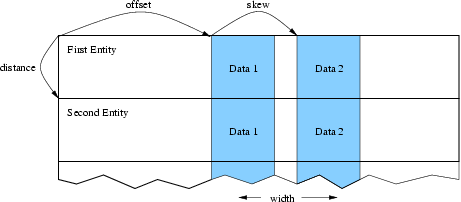
\includegraphics[width=5in]{fig/layout}
\end{center}
\caption{Describing a complex data layout.}
\label{fig:layout}
\end{figure}

For example, if your node data is all stored in a struct (in fortran, a named TYPE), offsetBytes gives the distance between the start of the struct and the force; and distanceBytes gives the size in bytes of the struct.  

In C, the offsetof and sizeof keywords are useful for finding these values.  In Fortran, we provide a special routine called \kw{foffsetof} that returns the distance, in bytes, between its two arguments.

\begin{alltt}
// C++ version:
     typedef struct \{
        double d[3], v[3], force[3], a[3];
        double m;
     \} node;
     node *nodes=new node[n];
     IDXL\_Layout\_t force\_layout=IDXL\_Layout\_offset(IDXL\_DOUBLE,3,
              offsetof(node,force),sizeof(node),0);

! F90 Version
     TYPE node 
        DOUBLE PRECISION :: d(3), v(3), force(3), a(3)
        DOUBLE PRECISION :: m
     END TYPE
     integer :: force\_layout
     ALLOCATE(nodes(n))
     force\_layout=IDXL\_Layout\_create(IDXL\_DOUBLE,3,
   &          foffsetof(nodes(1),nodes(1)\%force),
   &          foffsetof(nodes(1),nodes(2)),0)
\end{alltt}


\prototype{IDXL\_Layout\_destroy}
\function{void IDXL\_Layout\_destroy(IDXL\_Layout\_t layout);}
\function{SUBROUTINE IDXL\_Layout\_destroy(layout)}
  \args{INTEGER, INTENT(IN)  :: layout}

Destroy this Layout.  You only need call this routine if you repeatedly create layouts.

\prototype{IDXL\_Get\_layout\_type}
\function{int IDXL\_Get\_layout\_type(IDXL\_Layout\_t layout);}
\function{INTEGER function IDXL\_Get\_layout\_type(layout)}

Return the IDXL datatype for this layout.

\prototype{IDXL\_Get\_layout\_width}
\function{int IDXL\_Get\_layout\_width(IDXL\_Layout\_t layout);}
\function{INTEGER function IDXL\_Get\_layout\_width(layout)}

Return the layout width---the number of data items that are communicated
per entity.

\prototype{IDXL\_Get\_layout\_distance}
\function{int IDXL\_Get\_layout\_distance(IDXL\_Layout\_t layout);}
\function{INTEGER function IDXL\_Get\_layout\_distance(layout)}

Return the layout distance---the number of bytes between successive
entity's data items.



\subsubsection{Layout Compatability Routines}

Before IDXL was made a separate library, FEM included these routines,
which are still preserved for backward compatability.

\prototype{FEM\_Create\_simple\_field}
\function{IDXL\_Layout\_t FEM\_Create\_simple\_field(int type,int width);}
\function{INTEGER function FEM\_Create\_simple\_field(type,width)}
  \args{INTEGER, INTENT(IN)  :: type,width}

This routine is completely interchangable to \kw{IDXL\_Layout\_create}.


\prototype{FEM\_Create\_field}
\function{int FEM\_Create\_field(int type,int width,int offset,int distance);}
\function{INTEGER function FEM\_Create\_field(type, width, offset, distance)}
  \args{INTEGER, INTENT(IN)  :: type, width, offset, distance}

This routine is like a call to \kw{IDXL\_Layout\_offset} with the rarely
used \kw{skewBytes} set to zero.



%%%%%%%%%%%%%%%%%%% Communication %%%%%%%%%%%%%%%%%%%%
\subsection{IDXL Communication}
\label{sec:IDXLComm}
This section brings together all the pieces of IDXL: Index Lists are used to determine what to send and what to receive and Layouts are used to determine where to get and put the communicated data.


\subsubsection{Communication Routines}

\prototype{IDXL\_Comm\_sendsum}
\function{void IDXL\_Comm\_sendsum(IDXL\_Comm\_t comm,IDXL\_t indices,IDXL\_Layout\_t layout,void *data);}
\function{SUBROUTINE IDXL\_Comm\_sendsum(comm,indices,layout,data)}
  \args{INTEGER, INTENT(IN)  :: comm,indices,layout}
  \args{varies, INTENT(INOUT) :: data}

Sum these \kw{indices} of shared entites across all chunks that share them.
The user \kw{data} array is interpreted according to the given \kw{layout}.

If \kw{comm} is zero, this routine is blocking and finishes the communication immediately.
If \kw{comm} is not zero, this routine is non-blocking and equivalent to a call to 
\kw{IDXL\_Comm\_send} followed by a call to \kw{IDXL\_Comm\_sum}.

This routine is typically used to sum up partial values on shared nodes.
It is a more general version of the old FEM routine \kw{FEM\_Update\_field}.
For example, to sum up the shared-node values in a 3d \uw{force} vector indexed 
by node, you would use:

\begin{alltt}
// C++ version:
     double *force=new double[3*nNodes];
     IDXL\_Layout\_t force\_layout=IDXL\_Layout\_create(IDXL\_DOUBLE,3);
     IDXL\_t shared\_indices=FEM_Comm_shared(mesh,FEM_NODE);
     
     ... in the time loop ...
         IDXL_Comm_sendsum(0,shared_indices,force_layout,force);

! F90 Version
     double precision, allocatable :: force(:,:)
     integer :: force\_layout, shared_indices
     ALLOCATE(force(3,nNodes)) ! (could equivalently use force(3*nNodes) )
     force\_layout=IDXL\_Layout\_create(IDXL\_DOUBLE,3)
     shared_indices=FEM_Comm_shared(mesh,FEM_NODE)
     
     ... in the time loop ...
         CALL IDXL_Comm_sendsum(0,shared_indices,force_layout,force)

\end{alltt}


\prototype{IDXL\_Comm\_sendrecv}
\function{void IDXL\_Comm\_sendrecv(IDXL\_Comm\_t comm,IDXL\_t indices,IDXL\_Layout\_t layout,void *data);}
\function{SUBROUTINE IDXL\_Comm\_sendrecv(comm,indices,layout,data)}
  \args{INTEGER, INTENT(IN)  :: comm,indices,layout}
  \args{varies, INTENT(INOUT) :: data}

Send these (typically real) send \kw{indices} and copy in these 
(typically ghost) receive \kw{indices}.
The user \kw{data} array is interpreted according to the given \kw{layout}.

If \kw{comm} is zero, this routine is blocking and finishes the communication immediately.
If \kw{comm} is not zero, this routine is non-blocking and equivalent to a call to 
\kw{IDXL\_Comm\_send} followed by a call to \kw{IDXL\_Comm\_sum}.

This routine is typically used to obtain the values of ghost entities.
It is a more general version of the old FEM routine \kw{FEM\_Update\_ghost\_field}.
For example, to obtain 7 solution values per ghost element, storing \uw{gElem}
ghosts in the array just after the \uw{nElem} regular elements, we could:

\begin{alltt}
// C++ version:
     double *elem=new double[7*(nElem+gElem)];
     IDXL\_Layout\_t elem\_layout=IDXL\_Layout\_create(IDXL\_DOUBLE,7);
     IDXL\_t ghost\_original=FEM_Comm_ghost(mesh,FEM_ELEM+1);
     IDXL\_t ghost\_shifted=IDXL_Create(); // ghosts start at nElem
     IDXL_Combine(ghost_shifted,ghost_original,0,nElem);
     
     ... in the time loop ...
         IDXL_Comm_sendrecv(0,ghost_shifted,elem_layout,elem);

! F90 Version
     double precision, allocatable :: elem(:,:)
     integer :: elem\_layout, ghost_original,ghost_shifted
     ALLOCATE(elem(7,nElem+gElem))
     elem\_layout=IDXL\_Layout\_create(IDXL\_DOUBLE,7)
     ghost\_original=FEM_Comm_ghost(mesh,FEM_ELEM+1)
     ghost\_shifted=IDXL_Create() ! ghosts start at nElem+1
     CALL IDXL_Combine(ghost_shifted,ghost_original,1,nElem+1)
     
     ... in the time loop ...
         CALL IDXL_Comm_sendrecv(0,ghost_shifted,elem_layout,elem)

\end{alltt}


\subsubsection{Advanced Communication Routines}

\prototype{IDXL\_Comm\_begin}
\function{IDXL\_Comm\_t IDXL\_Comm\_begin(int tag,int context);}
\function{INTEGER function IDXL\_Comm\_begin(tag,context)}
  \args{INTEGER, INTENT(IN)  :: tag,context}

Start a non-blocking communication operation with this (user-defined) tag and communication context (0, or an AMPI communicator).  

Every call to this routine must eventually be matched by a call to \kw{IDXL\_Comm\_wait}.  Warning: for now, tag and context are ignored, and there can be only one outstanding communication operation.


\prototype{IDXL\_Comm\_send}
\function{void IDXL\_Comm\_send(IDXL\_Comm\_t comm,IDXL\_t indices,IDXL\_Layout\_t layout,const void *data);}
\function{SUBROUTINE IDXL\_Comm\_send(comm,indices,layout,data)}
  \args{INTEGER, INTENT(IN)  :: comm,indices,layout}
  \args{varies, INTENT(IN) :: data}

When \kw{comm} is flushed, send these send \kw{indices}, with
this \kw{layout}, from this \kw{data} array.

This routine is always non-blocking; as the \kw{data} array passed in
will not be copied out until the call to \kw{IDXL\_Comm\_flush}.


\prototype{IDXL\_Comm\_recv}
\function{void IDXL\_Comm\_recv(IDXL\_Comm\_t comm,IDXL\_t indices,IDXL\_Layout\_t layout,void *data);}
\function{SUBROUTINE IDXL\_Comm\_recv(comm,indices,layout,data)}
  \args{INTEGER, INTENT(IN)  :: comm,indices,layout}
  \args{varies, INTENT(OUT) :: data}

When \kw{comm} is finished, copy in these receive \kw{indices}, with
this \kw{layout}, into this \kw{data} array.

This routine is always non-blocking; as the \kw{data} array passed in
will not be copied into until the call to \kw{IDXL\_Comm\_wait}.


\prototype{IDXL\_Comm\_sum}
\function{void IDXL\_Comm\_sum(IDXL\_Comm\_t comm,IDXL\_t indices,IDXL\_Layout\_t layout,void *data);}
\function{SUBROUTINE IDXL\_Comm\_sum(comm,indices,layout,data)}
  \args{INTEGER, INTENT(IN)  :: comm,indices,layout}
  \args{varies, INTENT(INOUT) :: data}

When \kw{comm} is finished, add in the values for these receive \kw{indices}, 
with this \kw{layout}, into this \kw{data} array.

This routine is always non-blocking; as the \kw{data} array passed in
will not be added to until the call to \kw{IDXL\_Comm\_wait}.


\prototype{IDXL\_Comm\_flush}
\function{void IDXL\_Comm\_flush(IDXL\_Comm\_t comm);}
\function{SUBROUTINE IDXL\_Comm\_flush(comm)}
  \args{INTEGER, INTENT(IN)  :: comm}

Send all outgoing data listed on this \kw{comm}.  This routine exists because there may be many calls to \kw{IDXL\_Comm\_send}, and sending one large message is more efficient than sending many small messages.

This routine is typically non-blocking, and may only be issued at most once per \kw{IDXL\_Comm\_begin}.


\prototype{IDXL\_Comm\_wait}
\function{void IDXL\_Comm\_wait(IDXL\_Comm\_t comm);}
\function{SUBROUTINE IDXL\_Comm\_wait(comm)}
  \args{INTEGER, INTENT(IN)  :: comm}

Finish this communication operation. This call must be issued exactly once per \kw{IDXL\_Comm\_begin}.  This call inclues \kw{IDXL\_Comm\_flush} if it has not yet been called.

This routine always blocks until all incoming data is received, and is the last call that can be made on this \kw{comm}.

